\documentclass[main.tex]{subfiles}
\begin{document}

\marginpar{Tuesday\\ 2021-11-9, \\ compiled \\ \today}

As a reminder, the Lorentz factor can be written as \(\gamma = E / mc^2\), while the  
factor \(\beta \) can be written as \(\beta = \abs{\vec{p}} c / E\). 

Now we move to natural units: \(\hbar = c = 1\). 

We come back to our decay \(M \to m_1 + m_2 \). 
We have computed the CoM energies and momenta, now we need
to move back to the lab frame. 
The Lorentz transformation with \(- \beta \) reads 
%
\begin{subequations}
\begin{align}
\left[\begin{array}{c}
E_i \\ 
p_{i, \parallel}
\end{array}\right]
&= \left[\begin{array}{cc}
\gamma  & \gamma \beta  \\ 
\gamma \beta  &  \gamma 
\end{array}\right] 
\left[\begin{array}{c}
E_{i}^{*} \\ 
p_{i}^{*} \cos \theta^{*}
\end{array}\right]  \\
&= 
\left[\begin{array}{c}
\gamma \qty(E_i^{*} + \beta p^{*} \cos \theta^{*}) \\ 
\gamma \qty(\beta E_i^{*} + p^{*} \cos \theta^{*})
\end{array}\right]
\,.
\end{align}
\end{subequations}

The emission angles may change depending on the interaction, so the \(\theta^{*}\) dependence is relevant. 

We can recover the emission angle in the lab frame by 
%
\begin{align}
\tan \theta_i = \frac{p_{i, \perp}}{p_{i, \parallel}}
= \frac{p_i^{*} \sin \theta^{*}}{\gamma \qty(\beta E_i^{*} + p_i^{*} \cos \theta^{*})}
\,.
\end{align}

Even if the emission is isotropic in the CoM frame, it will not be in the lab frame; qualitatively, it will be peaked in the forward direction. 

If \(\theta^{*} = 0\), we get \(\theta = 0\).
If \(\theta^{*}= \pi /2\), we get 
%
\begin{align}
\tan \theta = \frac{1}{\gamma } \frac{p^{*}}{\beta E_i^{*}}
= \frac{1}{\gamma } \frac{\beta^{*}_i}{\beta^{*}}
\,.
\end{align}

In the ultrarelativistic limit, this will be \(\sim 1/ \gamma \): therefore, we will get \(\theta \sim \arctan (1 / \gamma ) \sim 1/ \gamma \).

\begin{figure}[ht]
\centering
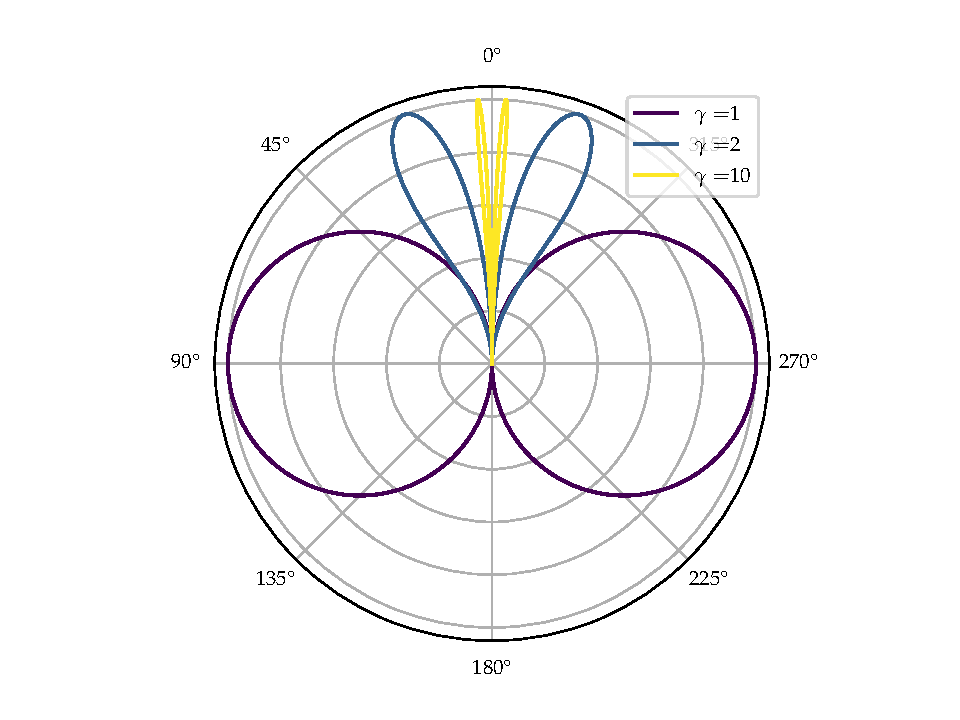
\includegraphics[width=\textwidth]{figures/angular_distribution_shift}
\caption{Angular distribution of the emitted radiation if the starting emission is isotropic, which means that the probability distribution for \(\theta^{*} \) is \(\dd{p} = \sin \theta^{*} \dd{\theta^{*} }\), which corresponds in the plot to the \(\gamma = 1\) case. Here we are assuming that the decay looks like \(1 \to 2 +3 \), where both 2 and 3 are massless.
We also show the \(\theta \sim 1/\gamma \) approximation as a dashed line. In the high \(\gamma \) limit, this is the median of the distribution.}
\label{fig:angular_distribution_shift}
\end{figure}

Let us consider the decay of a neutral pion: 
%
\begin{align}
\pi^{0} \to \gamma + \gamma 
\,.
\end{align}

In the CoM system, both photons will get \(E^{*} = M/2 = p^{*}\), where \(M = m_{\pi^{0}} \approx \SI{134.98}{MeV}\).

The lab-frame energy of one of these is given by 
%
\begin{subequations}
\begin{align}
E &= \gamma \qty(E^{*} + \beta p^{*} \cos \theta^{*})\\
 &= \gamma E^{*} ( 1 + \beta \cos \theta^{*})  \\
 &= \frac{E_\pi }{m_\pi } \frac{m_\pi}{2} \qty(1 + \beta \cos \theta^{*})  \\
 &= \frac{E_\pi }{2} \qty(1 + \beta \cos \theta^{*})
\,.
\end{align}
\end{subequations}

The maximum of this quantity is \(E_\pi (1 + \beta ) /2\); its minimum is \(E_\pi (1 - \beta ) / 2\). 
This is just a bit smaller than the distribution \(E \in [0, \pi ]\). 

What is the distribution of the photons we get in the lab frame? How wide will the detector need to be? 
Well, we can frame it by selecting the size we need to get a certain high percentage of the emitted photons. 

An order-of-magnitude estimate is: half of the photons are emitted with \(\theta^{*} < \pi /2\), and their angle will be \(\lesssim 1 / \gamma \).

The original \(J/\psi \) papers are in the drive --- add citation.

\subsubsection{A \(1 \to 3\) decay example}

Now the three emitted particle momenta in the CoM frame will satisfy 
%
\begin{align}
\vec{p}^{*} _{\text{tot}} = 
p^{*}_{1} + 
p^{*}_{2} + 
p^{*}_{3} = 0
\,.
\end{align}

We define \(\theta^{*}\) as \(\theta^{*}_1\); the trick to solving this problem is to ``bunch'' particles \(2\) and \(3\) into one, with momentum \(\vec{p}^{*}_{23} = p^{*}_{2} + p^{*}_{3}\). 
The invariant mass of this system will read 
%
\begin{subequations}
\begin{align}
m_{\text{23}} &= \sqrt{p_2^2 + p_3^2 + 2 p_2 \cdot p_3}  \\
&= \sqrt{m_2^2 + m_3^2 + 2 E_2^{*} E_3^{*} - 2 \abs{p_2^{*}} \abs{p_3^{*}} \cos \theta^{*}_{23}}
\,,
\end{align}
\end{subequations}
%
where \(\theta^{*}_{23}\) is the angle between 2 and 3 in the CoM frame. 

We can recurse back to the 2 body formulas for the behaviour of the 1 and 23 system: the energy of 1 will be 
%
\begin{align}
E_1^{*} &= \frac{M^2 + m_1^2 - m_{23}^2}{2M}
\,.
\end{align}

Now, even in the CoM frame the energy of particle 1 (which is arbitrary) depends on the emission angle \(\theta^{*}_{23}\). 
We can, however, compute the minimum and maximum values of \(E_1^{*}\).

There is a ``trick'' which allows us to skip the whole computation. 
The idea is that \(m_{23} \) will be maximum when the most energy will be given to the 23 system; so this happens when \(m_1 \) is produced at rest, while the other two are back-to-back. 

Then, we will have \(p^{*}_2 = -p^{*}_3\). 

In this case, we will have \(m_{23}^{\text{max}} = M - m_1 \). It's as if both particles (1 and the ``combined particle'' 23) were produced at rest. 

In this case, then, 
%
\begin{align}
E^{*}_{1, \text{min}} &= \frac{M^2 + m_1^2 - (M^2 + m_1^2 - 2 M m_1 )}{2M} = m_1
\,,
\end{align}
%
as expected. 

The other extreme happens when \(m_{23} = m_2 + m_3 \); in this case, then, there must exist a frame in which both particles are at rest. 
This means that they must travel with the same velocity. 
This does not mean that the momenta are equal, in general \(p^{*}_2 \neq p^{*}_3\), but \(\vec{v}^{*}_2 = \vec{v}^{*}_3\).

The maximum energy is therefore 
%
\begin{align}
E^{*}_{1, \text{max}} = \frac{M^2 + m_1^2 - (m_2 + m_3 )^2}{2 M }
\,.
\end{align}

The most famous example here is \(\beta \) decay: from a nuclear perspective it is 
%
\begin{align}
N(A, Z) \to N(A, Z+1) + e^{-} + \overline{\nu}_e
\,,
\end{align}
%
since from a microphysical perspective what happened was
%
\begin{align}
\ce{n} \to \ce{p} + e^{-} + \overline{\nu}_{e}
\,.
\end{align}

Proton decay has not been observed, but \(\beta^{+}\) decay can happen since the nucleus is also involved. 

In the lab system, which is also the CoM system, we will have a minimum energy of \SI{511}{keV}, and a maximum energy of roughly \SI{1.29}{MeV}, which comes from the approximation 
%
\begin{align}
E _{e, \text{max}} \approx \frac{M^2(A, Z) - M^2 (A, Z+1)}{2 M(A, Z)}
\,.
\end{align}

If the neutrino were massive, this maximum of the distribution will be shifted down a bit.
This is an experimental challenge, since the mass of the neutrino is at most on the \SI{}{eV} scale. 

Let us consider the decay \(\pi^{-} \to \mu^{-} + \overline{\nu}_\mu \). 

The decay \(\pi^{-} \to e^{-} + \overline{\nu}_e\) is forbidden by the handedness of weak interactions. 
The helicity is conventionally positive for antiparticles and negative for particles. 

As a first approximation, if the antineutrino is going to the left and the electron is going to the right, both spins will be to the left, summing to 1 to the left, while the pion has spin 0. 

This is also the case for decay towards muons, but \(m_\mu \gg m_e\), therefore the probability for the muon to have a spin component to the right is much higher. 

\end{document}
